\chapter{Conclusion}
In this thesis a solution to the scalability problem of classical RSA-based group sharing scheme was given with respect to not violate any security requirements \ref{sec:requirements} that where already present in the reference system. Classical systems suffer from many file-keys that need to be maintained each time a new file is updated or a new member joins a group. Existing members need to make sure that the newly joined member can access all previous shared files by decrypting all file-keys and encrypting them again with the new members public key, creating own file keys for the new member. If a new file is updated, it need to made accessable to all members in the group. A file need to be encrypted one by one for each public key in the group. Creating $n$ more file-keys per file upload.

Different approaches are analyzed and argumentatively compared to end-up with an MA-ABE scheme fits the requirements and solves the scalability problem the best.  MA-ABE uses attribute to create an access policy under which a file is secured. This access policy acts like a shared group key that is only accessible to the members that satisfy this access policy. In that way does MA-ABE solves the initial problem of creating $n$ file keys per new file update. Each scheme using a group key only needs to encrypt the file once using the group key resulting in one shared file-key. 

MA-ABE was chosen as the best candidate, because it, in comparison to other secure-group communications, does not redistribute the shared group key to other members. The main feature of an ABE scheme is that the users inherently possesses all needed information to calculate the group key from their given attribute secrets. 

MA-ABE is especially important in the field of applied ABE schemes, since it divides the universe of attributes into different separated clusters, each managed and maintained by an own, self-organized AA. This breaks up a disadvantage of classical ABE schemes: the global decryption power of the system administrator or single AA. 

From the current field of MA-ABE schemes TF-DAC-MACS was the candidate that showed great scalability and performance, no global decryption power of the CA and a mechanism to revoke users from the system. Since it does not support 1-of-n threshold gate policies (OR-gates), an improved version to this scheme, called \name, was constructed and implemented. To further make \name more practically applicable the fix two-factor constrain was made optional. 

To evaluate whether \name indeed scales better than the classical rekeying scheme different benchmarks were performed against a reference implementation of the classical RSA-based rekeying scheme. The outcome was that regarding the number of file-keys \name scales better with a worst-case scenario were \name scales in the same way as the reference implementation. However, it was noticeable that this feature comes with additional overhead in file-key size. Taking this observation into account archives the prototype a better scalability when at most $n/2$ "OR"-gates are used in the access policy. 

Regarding performance a completely different picture is drawn. Due to the assumption that the number of attributes to describe a group is equal or less to the number of users in the group \name shows a better performance since it only works with the attributes and not the users directly. Depending on the underlying system and the chosen distribution of attributes to users an intersecting point can be calculated when \name shows a better performance. This intersecting point is located in the best-case scenario (Figure \ref{fig:1-for-infty-and}) at around 145 users. 

To achieve a better single encryption performance than the classical system at least 145 users need to be describable with one attribute. The resulting implication is that \name benefits from large scale systems with a lot of users that share a lot of attributes. Small groups that share perform peer-to-peer sharing suffer more from the additional overhead. Here \name can only be beneficial if storage and not computing power is the bottleneck. 

\section{Practical Applicability}

\begin{figure}[!ht]
\centering
    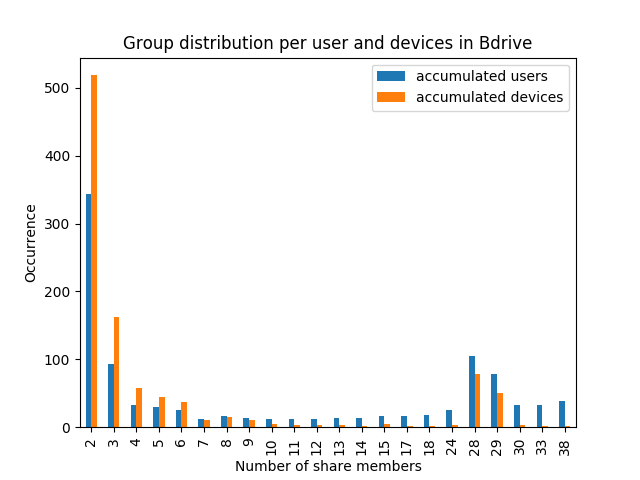
\includegraphics[width=1.0\linewidth]{img/share_distribution_bdirve.png}
    \caption{The distribution of shared folders per users and their aggregated devices.}
    \label{fig:evaluation-share-distribution}
\end{figure}

In the evaluation capture \ref{sec:evaluation} it was concluded that in the best-case scenario \name performs and scales better than the Bdrive from 145 users in a group onwards if they all can be described by the same attribute. To validate that is a common scenario in the real world the distribution of groups and their members of Bdrive are listed in Figure \ref{fig:evaluation-share-distribution}.

As it can be extracted from the figure, many users share file only to one or two other users. In that case would \name provide no performance  advantage. Really interesting for the ABE use case is the second spike at 28 to 30 members. Since Bdrive is addressed to business it can be assumed that this second spike define the company wide shared folders. It can be expected that for very large scale companies that have more then 300 employees. If they all are members in the same share/name can use its full potential, since all members will share a common attribute: "Employee in Company X".

In conclusion \name can reduce the number of file-keys dramatically if combined with the right access policy. It depends on the company administrator to assign each user suitable attributes so that fine-grain access formulas without using "OR"-gates can be constructed.  

\section{Future Work}
As shown in this work, ABE has the potential to improve today's applied cryptography. However, several improvements can be conducted to make \name better practically applicable.

\subsubsection{Handle Attributes On Device Level}
In the prototype attributes are handled on user level. Intuitively, that makes sense. Users are assigned to attributes and not something else. A much better approach would be to handle attributes on device level. In that way a user can more fine-graint define which device should be able to decrypt which data. For example, very sensitive information should not leave the company building and in turn not be decryptable by mobile devices. 

\subsubsection{Multible Two-Factor Keys}
Another missed opportunity to make the scheme more expressive was to be able to create different two-factor private keys. In the current implementation two-factor private keys are identified and bound by the user ID who created the cipher-text. That behavior was defined by TF-DAC-MACS and directly applied to \name. Since there always can just be one two-factor key per user, the number of possible two-factor keys are limited to the universe of users.

An more scalable way of defining two-factor keys would be to let each user create as many two-factor private key as he can. In theory this should be simply possible by providing each ciphertext a different two-factor private key on encryption. Users that want to decrypt this cipher text extract from the cipher-text the ID and version of the used two-factor key, check whether they have a suitable secret key and decrypt the cipher-text normally. 

\subsubsection{AA as a Client-Service}
To eliminate the need of having the AA always available it is possible to implement it as a client. In that way it would reduce the security risked of being exposed to the outer world. Such a system can be implemented if the central server is used as message broker. Since the thread model that the central server is untrusted but follows the protocol, each message that is send to the central server need to be authenticated by a signature. 

A set of trusted certificates can be installed at the client on bootstrapping it in a trusted environment. In that way it is ensured that only authentic signatures are accepted. This procedure comes with additional overhead on revoking one of this certificates. 

To prevent replay attacks clients (devices) can additionally also be bootstrapped with a random seed. This seed is only known to the client and the owning AA. Each seed for each device should be different. This seed can be feed into a pseudo-random function which produces a stream of random numbers. Each number will be included to the next message that will be exchanged and signed by the sender. In that way replay attacks of the central server can be mitigated, since the central server never knows which nonce will come next. The owning AA can just its known seeds and the public key of each device to distribute new seeds and onboard new AA that are trusted as well. 

\subsubsection{Fine-Graint Access Control}
In this work a very easy adaptation to DNF-access policies was given. Different access policies are build over the same file key so that if a user can decrypt one of the cipher text he can decrypt the file. In that way \name is able to support DNF-access formulas with the trade-off for performance and storage consumption.  

A much better way would be to embed the access formula directly into the cipher-text as it is also done with AND-gates. TF-DAC-MACS uses multiplicative terms that substitute each other if combined with the right secret keys to reveal the underlying secret. Other approaches in the field of MA-ABE support fine-graint access formulas already such as \cite{liu2016practical} \cite{yang2013dac} \cite{lewko2011decentralizing}. They utilize a technique called \textit{Linear Secret Sharing Scheme} (\ac{LSSS}). LSSS produces a matrix where each row correlates to a Boolean variable. An LSSS matrix is just a different and computationally more efficient way to display Boolean access trees. 

An input configuration $\vec{v}$ statisfy the LSSS matrix $A$ and if and only if 
$A\vec{v} = \begin{pmatrix}1 & 0 & \dots & 0 \end{pmatrix}^T$. \cite{liu2010efficient}. This behavior can be embedded into the cipher text to only reveal the secret if $A$ is satisfied. An disadvantage when using LSSS is that the underlying matrix will grow in complexity when defining more and more complex access policies. Exactly this point was improved by TF-DAC-MACS with the trade-off of only supporting n-of-n threshold gates. 

Having fine-grained access control implemented in the system would greatly improve the value of such system. Arbitrary monotone-access structures would enable to include numerical attributes into the system. In addition the number of file keys can be reduced to one regardless of the access policy. Here additional evaluation need to be conducted to analyze whether the trade-off for cipher-text size is negligible. 

\subsubsection{Automatically Compose Access Policies}
To be fully piratically applicable a algorithm must be developed that automatically calculates the access policy with the least overhead given a user group. For the normal user only very simple access policies are sizable. Such as "Works in company X" or "Is full-time employed". 
But sometimes users want to share files with specific users. They face the problem of not knowing which attributes they own and who will also be accidentally included in the group without them knowing. Most likely user will fall back to use explicit OR-policies to prevent this case from happening. As the reader can the a lot of worst-case access policies might be created. 

An algorithm can help here. Such an algorithm can analyzed the given user group and find the smallest intersecting subset of attributes that are needed to completely define this group and without including any unwanted members. If no such excluding policy can be constructed the algorithm could either create an group defining attribute (same overhead as secure group communications) or fall back to the worst-case access policy (same overhead as the classical rekeying scheme). 

\section{Summary}
In this thesis an new MA-ABE scheme was presented that used TF-DAC-MACS as a base line. It was shown that such a secure cloud storage system utilizing \name can exist in practice. The proposed scheme is able to reduce the number of file keys, depending on the chosen access policy, to a minimum. Such a system comes with the trade-off of performance and a bigger storage overhead per file-key. Different evaluations are conducted to find the point where \name scales better then the current implemented solution of a secure cloud storage system. For the most encryptions and member join operations this point can be found, while this system comes with an additional overhead on member-leave operations. The member-leave operation can be highly parallized which leads to the conclusion that \name is ready to be practical evaluated in a real world system. 

Here open question remain: Since ABE schemes include the user level attributes into the cryptography administrator and user need to adapt in the way they handle attributes and address users. Administrators need to define attributes in that way that groups are usually describable by one attribute to use ABE efficiently. Users on the other hand need to understand that they address encrypted files to an attribute policy rather then to individuals. This last point can be transparently hidden by algorithm that automatically calculate the most efficient access policy. But the fact remains that an ABE system can only be used effectively and efficient if all participants interact not individual, but on an descriptive attribute level with each other. 

